\documentclass[11pt, fullpage,letterpaper]{article}

\usepackage[margin=1in]{geometry}
\usepackage{url}
\usepackage{amsmath}
\usepackage{float}
\usepackage{graphicx}
\usepackage{times,amsmath,amsthm,amsfonts,eucal,graphicx}
\usepackage{hyperref}

\newcommand{\assignmentId}{1}

\newcommand{\bx}{{\bf x}}
\newcommand{\bw}{{\bf w}}

\renewcommand{\cite}[1]{[#1]}
\def\beginrefs{\begin{list}%
        {[\arabic{equation}]}{\usecounter{equation}
         \setlength{\leftmargin}{2.0truecm}\setlength{\labelsep}{0.4truecm}%
         \setlength{\labelwidth}{1.6truecm}}}
\def\endrefs{\end{list}}
\def\bibentry#1{\item[\hbox{[#1]}]}



\title{Biodiversity Clustering}
\author{Jadon Wagstaff and Christian Felt}

\begin{document}

	\maketitle
	
	\section{Introduction}
		Data was obtained from the International Union for the Conservation of Nature (IUCN) via shapefiles [IUCN 17]. The files contained sets of polygons representing the ranges of different species assessed by the IUCN. We set out to explore methods of polygon clustering, and how we could use clustering to answer the questions:
		\begin{itemize}
			\item Where are areas of high biodiversity?
			\item Where are areas of high levels of species endangerment?
		\end{itemize} 
		We divided the work into two parts. Christian created centroids of each polygon and implemented clustering algorithms discussed in class (Sections 2.1, and 3). Jadon created a point cloud for the data, explored density based clustering methods, and developed a technique to identify density peaks and prominence (Sections 2.2, and 4).
	
	\section{Data}
	\subsection{Centroids}
		The data obtained was in the form of Esri shapefiles containing polygons. Each polygon was associated with a species identification number. These polygons were often large, diverse, complex, and overlapping. They proved to be unsuitable for our methods as they were. The first method used to mitigate these problems was to calculate centroids of the polygons using ArcMap software.
		
	\subsection{Point Cloud}
		The other method to ease calculations was to create an ordered set of points on the globe and find which were contained in the polygon, then use this point cloud for the clustering algorithms. To create a point cloud, we created an array of size $n$ with each row corresponded to a latitude from $-89.8^o$ to $89.8^o$ with a change of $.2^o$ latitude between each row. Each array contained an array of longitude elements from		 $-180^o$ to $180^0$ in increments of $\frac{.2}{\cos(latitude)}$. This gave about a million points in a grid like point cloud set with approximately $22km$ great-circle distance between adjacent points. For a given polygon, each point was assessed to determine whether it was contained in the polygon or not. This was accomplished by determining how many times a ray, starting at the point, intersected the polygon. Once it was determined that a point was in the polygon, the species id of that polygon was added to an array representing that point. This was done for all polygons and the result was an ordered point cloud, each an array of species found at that geographical coordinate. Each array has the property that the size of the array corresponds to the depth of polygons at that point. This set of points preserves more information about the shape and size of the polygon than centroids, and the fact that the point cloud is ordered was utilized to make the clustering algorithms more efficient.
		
		Another shortcoming of the data is that information about red-list status was missing. (Red-list status is essentially whether a species is endangered or not.) To supply the needed information, the IUCN database was queried for each species represented by polygons. After that the clustering algorithms were able to do clustering on the whole data set, or just polygons associated with species on the red-list. 
	
	\section{Using Clustering to Identify Hotspots}
		In this section, our goal was to determine whether the clustering techniques we learned in class could divide the ranges of endangered species into biologically reasonable groups. We assessed whether the clusters seemed biologically reasonable or not by comparing them to the areas of high biodiversity identified in the influential paper ``Biodiversity Hotspots for Conservation Priorities'' \cite{Myers 00}. Our conclusion was that Gonzalez clustering, simply by greedily choosing each new center to maximize the geographic distance from previous centers, was able to find biologically meaningful groups with a surprising degree of accuracy, though it also made notable errors, particularly where Myers's hotspots are located close together (in which case Gonzalez tended to combine them), or the density of endangered species was low (in which case Gonzalez tended to assign the species to clusters centered far away).
		 
		Using ArcMap software, we computed the centroids of the polygons that represent the ranges of terrestrial animals (mammals, amphibians, and reptiles) in the IUCN Endangered Species Red List shapefiles, making sure that the centroid was adjusted if necessary to lie within the polygon. Using our own Python code, we turned the latitude and longitude coordinates of these centroids into a 2-dimensional matrix and performed various kinds of clustering.
				
		To measure distance, we used the great-circle distance as given by d from the Haversine formula, where $\phi$ latitude, $\lambda$ is longitude, and $R$ is the radius of the Earth.
		\begin{equation}
			a = \sin^2 \frac{\Delta\phi}{2} + \cos \phi_1 (\cos \phi_2)  (\sin^2 \frac{\Delta\lambda}{2})
		\end{equation}
		\begin{equation}
			c =  \begin{cases} 
					0 & a = 0 \cr \tan^{-1}{\frac{\sqrt{1-a}}{a}} & a \neq 0
				\end{cases}
		\end{equation}
		\begin{equation}
			d = R*c
		\end{equation}
	
		Since the Earth is not perfectly spherical, the great-circle distance may be wrong by up to approximately 0.3\% or 22 km, according to user ``whuber's'' detailed analysis on gis.stackexchange \cite{whuber 12}. However, this error seems acceptable since in ``Global Patterns of Terrestrial Vertebrate Diversity and Conservation,'' Jenkins et al set 100 km as a reasonable lower limit for ``fine-grained spatial analysis'' in this field \cite{Jenkins 13}.
	
		Hierarchical clustering ran too slowly for the full centroid dataset (74,529 points) or for amphibians alone (18,694 points). K-means++ worked for small numbers of clusters (20 or less) but became obnoxiously slow for larger k. Lloyd's was also too slow for more than about 20 clusters. 
		
		Gonzalez clustering, however, processed the entire dataset in less than 10 seconds. Using the “elbow principle” (see Figure 3) and a subjective sense of how many clusters looked good on the final map (adopting a scale similar to Myers's), we chose k=40, and obtained the following clusters:

		\begin{figure}[H]
			\centering
			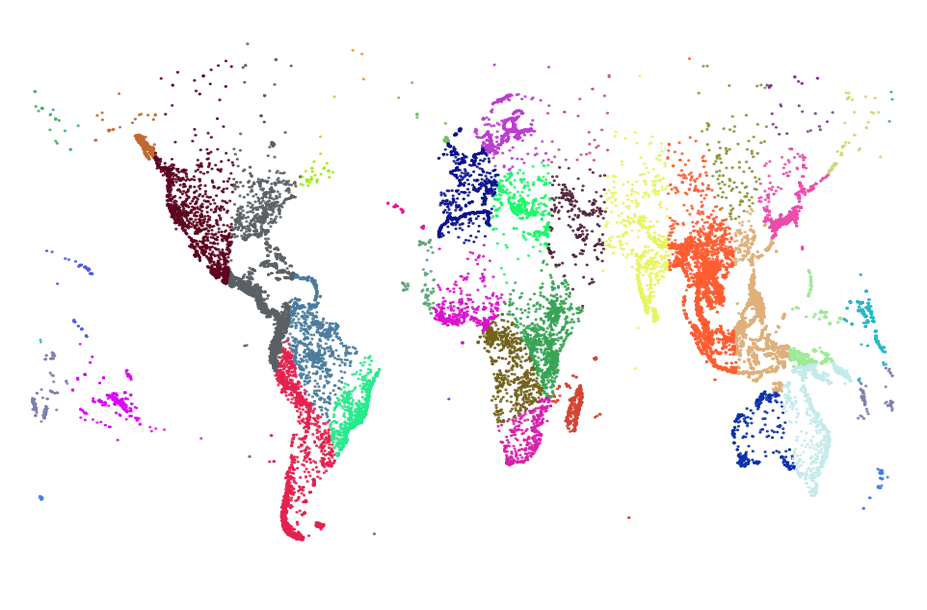
\includegraphics[width=11cm]{gonzalez.png}
			\caption{Gonzalez clusters with k = 40}
		\end{figure}
		
		\begin{figure}[H]
			\centering
			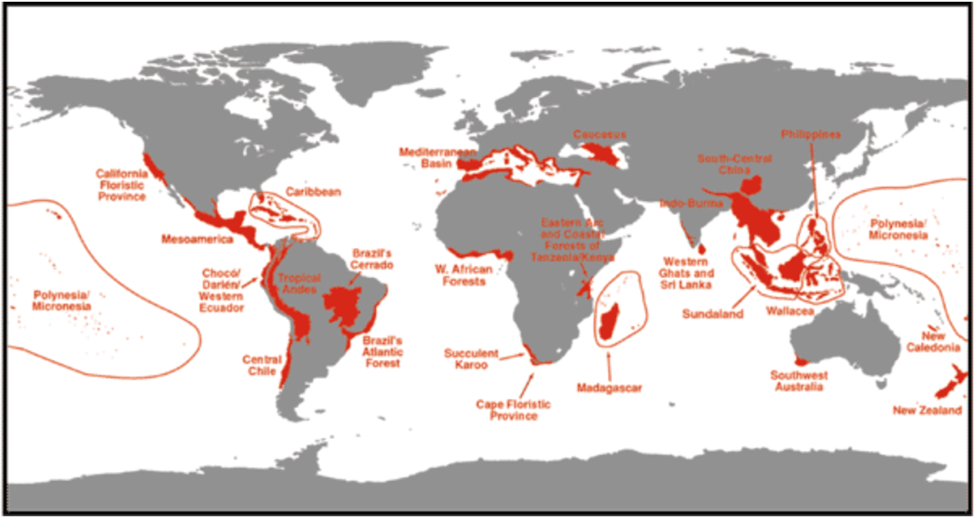
\includegraphics[width=11cm]{myers.png}
			\caption{Myers's 25 Biodiversity Hotspots}
		\end{figure}
		
		\begin{figure}[H]
			\centering
			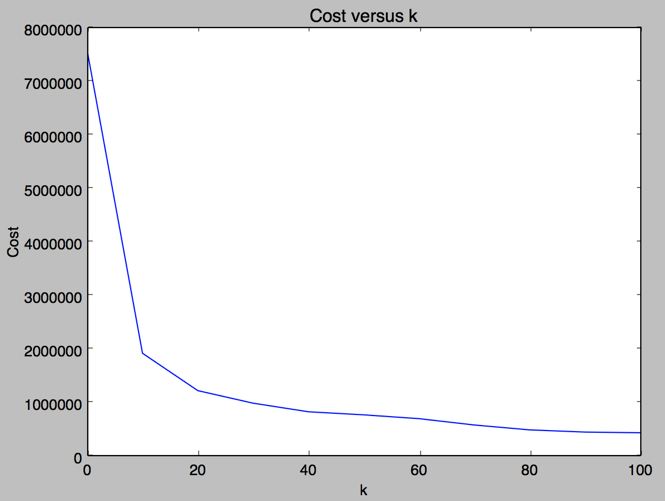
\includegraphics[width=7cm]{kMeansCost.png}
			\caption{k-means cost in meters for Gonzalez}
		\end{figure}
			
		These clusters seem surprisingly reasonable, rarely breaking up Myers's biodiversity hotspots (see Figure 2). According to Myers, ``[As many as] 35\% of all species in four vertebrate groups are confined to 25 hotspots comprising only 1.4\% of the land surface of the Earth...The hotspots’ boundaries have been determined by ‘biological commonalities’. Each of the areas features a separate biota or community of species that fits together as a biogeographic unit.'' It is interesting, then, that Gonzalez clustering, while taking into account nothing but geographic proximity, manages to pick out ``communities of species'' that are related in more biologically profound ways. For instance, Gonzalez, like Myers, assigns Madagascar, New Zealand, and the Caucasus Mountains to their own groups, separates the ``California Floristic Province'' from the rest of the Rockies, the ``West African Forests'' from the rest of Africa, and divides up the Indonesian Islands into three different groups, with the Philippines being mostly on their own. The Aleutian and Canary Islands, Newfoundland, and Hawaii are given their own clusters, and the Andes, Himalayas, and other mountain chains are not too broken up. 

		Sometimes, however, Gonzalez doesn't break groups up enough. It is blind to Myers's ``Succulent Karoo,'' located right next to ``Cape Floristic Province,'' and fails to separate the ``Central Chile'' or ``Western Ecuador'' hotspots from the larger ``Mesoamerica'' or ``Tropical Andes'' groups, respectively. Elsewhere, Gonzalez separates too much, for instance, breaking the Mediterranean Basin into two clusters. It is also wrong that Gonzalez has divided Siberia into so many strips (as if coinciding with Russia's many time zones.) This is a consequence of the low density of endangered species in Siberia; the data points there tend to be drawn into the clusters of distant, more densely-populated areas. A similar problem occurs in northern Canada and the Sahara.

		In summary, Gonzalez clustering provides a fast way to group endangered species in ways that make a surprising amount of biological sense. Since Gonzalez relies only on geographic distance, ``knowing'' nothing else about the animals, the explanation for why Gonzalez seems to be able to identify biological relationships must be that biological relationships are strongly conditioned by geographical proximity, and that the boundaries of terrestrial ecosystems are relatively discrete.
		
		Finally, we ran Gonzalez on the point cloud data (see Figure 4), even though our concern in this section has been the shape and location of clusters, not the density of species within them. In the point cloud, instead of having one point per species, each of the 534,809 points signifies the presence of any endangered species in the approximately 20 km by 20 km territory of which it is the center. On this expanded dataset, Gonzalez takes much longer (about 10 minutes), but the results are similar. Siberia and North America are still affected by arbitrary stripes. Species-poor areas, such as the Arabian, Sahara, and Central Asian deserts, show up even more dramatically (they're totally white.) The hotspots in the Pacific Northwest, Madagascar, New Zealand, and West African are still correctly identified, but the Mediterranean Basin is even more broken up, into 4 clusters rather than 2 (while Myers claims there should be only 1).
		
		In short, centroids seem to be a better modelling choice than the point cloud for locating hotspots, since their results are at least as good and they run much faster. One explanation for this is that a large proportion of endangered species in hotspots are unique to their areas; therefore, representing them by only one point, at the center of their habitat, should not result in as much loss of information as it would for more common species with larger or multiple ranges. 
		
		\begin{figure}[H]
			\centering
			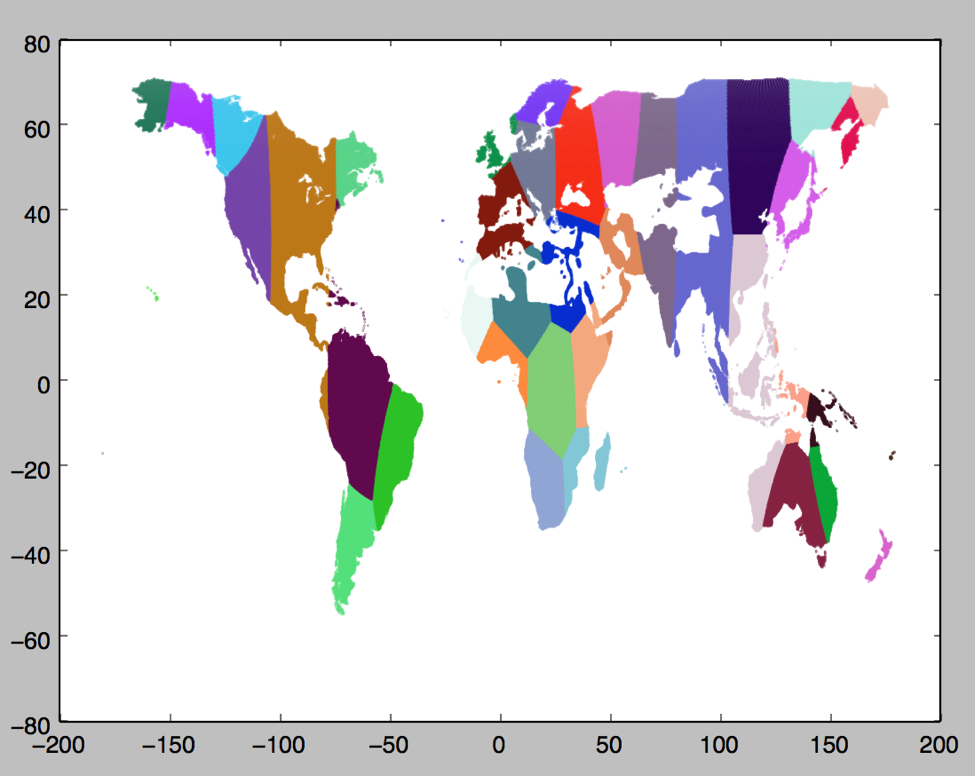
\includegraphics[width=10cm]{gonzalezPointCloud.png}
			\caption{Gonzalez clusters with k = 40 using the point cloud dataset}
		\end{figure}

	\section{Density Based Approach}
	\subsection{DBSCAN}
		Since we are asking to find where areas of greater biodiversity or greater endangerment are located, a density based clustering algorithm is a natural choice. Additionally, a paper on the topic \cite{Joshi 11} gives evidence that density based algorithms are good option for solving polygon clustering problems. Using the centroid data, the great circle distance metric, and suggestions from the paper \cite{Joshi 11}, an implementation of a modified version of dbscan was created in C++.
		\begin{tabbing}
			Mod\= ifie\= d db\= scan algorithm:\\
			\> Choose distance $\epsilon$ and number of points $minPts$\\
			\> Go to each data point and if it is unlabelled\\
			\> \> If the number of data points within $\epsilon$ is less than $minPts$\\
			\> \> \> label it outlier\\
			\> \> otherwise\\
			\> \> \> label it and all reachable core points as part of the same cluster\\
		\end{tabbing}

		A core point is a point with greater than $minPts$ number of points within an $\epsilon$ radius. This implementation differs from the normal dbscan because points are only included in a cluster if they qualify as a core point and they are within $\epsilon$ of a core point in the cluster. Run-time for the implementation on all  74,529 centroids was about half an hour. This implementation created clusters; however, the high density clusters do not match well with the diversity maps found on biodiversitymapping.org. This is the result of the centroid data losing too much information about the polygons.
		
		To improve results, an implementation of the modified dbscan for the ordered point cloud dataset was created. For this implementation, the density of an $\epsilon$ radius around a point $p$ was found by taking the average depth of $p$ and each point within $\epsilon$ of $p$. Also, $\epsilon$ was limited to values greater than $22km$ since no points were closer together than that. The resulting clusters matched nicely with maps on biodiversitymapping.org as long as $\epsilon$ was smaller than about $75km$.
		
		At this point, the polygons were able to be clustered for some depth threshold to provide regions where biodiversity or endangerment were above that threshold. Additionally, the depth information can be used to create a heat map of biodiversity. These are interesting, if somewhat trivial, tools to analyze the data. Now, is there a way to find and quantify the regions of high density relative to their surroundings? The next section addresses this question.
		
	\subsection{Cluster Prominence}
		In topological data analysis, persistent homology is used to detect prominent features of a space and the results are shown in a persistence diagram. The ideas found in persistent homology can be adapted to find regions of high density relative to their surroundings. Instead of building complexes by increasing the $\epsilon$ ball around a point, clusters are built by decreasing the $minPts$ value and keeping $\epsilon$ constant. And instead of killing complexes by merging them into older complexes, clusters are killed by merging them with denser clusters.
		
		\begin{tabbing}
			Mod\= ifie\= d db\= scan \= alg\= orithm with prominence calculation:\\
			\> choose distance $\epsilon$ and the maximum possible points, $max$, within any $\epsilon$\\
			\> for $minPts = max... 0$\\
			\> \> for each point $p$, if $p$ is unlabelled and a core point\\
			\> \> \> let $p$ and all reachable core points be in set $C$\\
			\> \> \> \> if all points in $C$ are unlabelled\\
			\> \> \> \> \> for cluster $c$, $birth(c) \leftarrow minPts$\\
			\> \> \> \> \> $\forall p_i \in C$, $label(p_i) = c$\\
			\> \> \> otherwise, choose $p_0 \in C$ s.t. $birth(p_0)$ is maximal\\
			\> \> \> \> for any labelled $p_i \in C$, if $label(p_i) \neq label(p_0)$\\
			\> \> \> \> \> $death(label(p_i)) \leftarrow minPts$\\
			\> \> \> \> \> $\forall p_i \in C$, $label(p_i) \leftarrow label(p_0)$\\
		\end{tabbing}
		
		All the clusters $c$ produced by the algorithm have a point, $(birth(c), death(c))$, that can be plotted on a $max(minPts) \times max(minPts)$ size graph.  to form a prominence diagram. Clusters with a high birth value are more dense than clusters with lower birth values. Further, $death(c)$ gives the lowest density that occurs between that point and the closest denser cluster. These can be used to find the prominence of a density cluster which is the distance between $(birth(c), death(c))$ and the diagonal. 
		
		To demonstrate the effectiveness of this approach, the results for mammal biodiversity are shown in the figures below. For each newly formed cluster, a point was generated by calculating the mean latitude and longitude for all points in the cluster at birth. The points corresponding to interesting points on the persistence diagram are highlighted on the map.
		
		\begin{figure}[H]
			\centering
			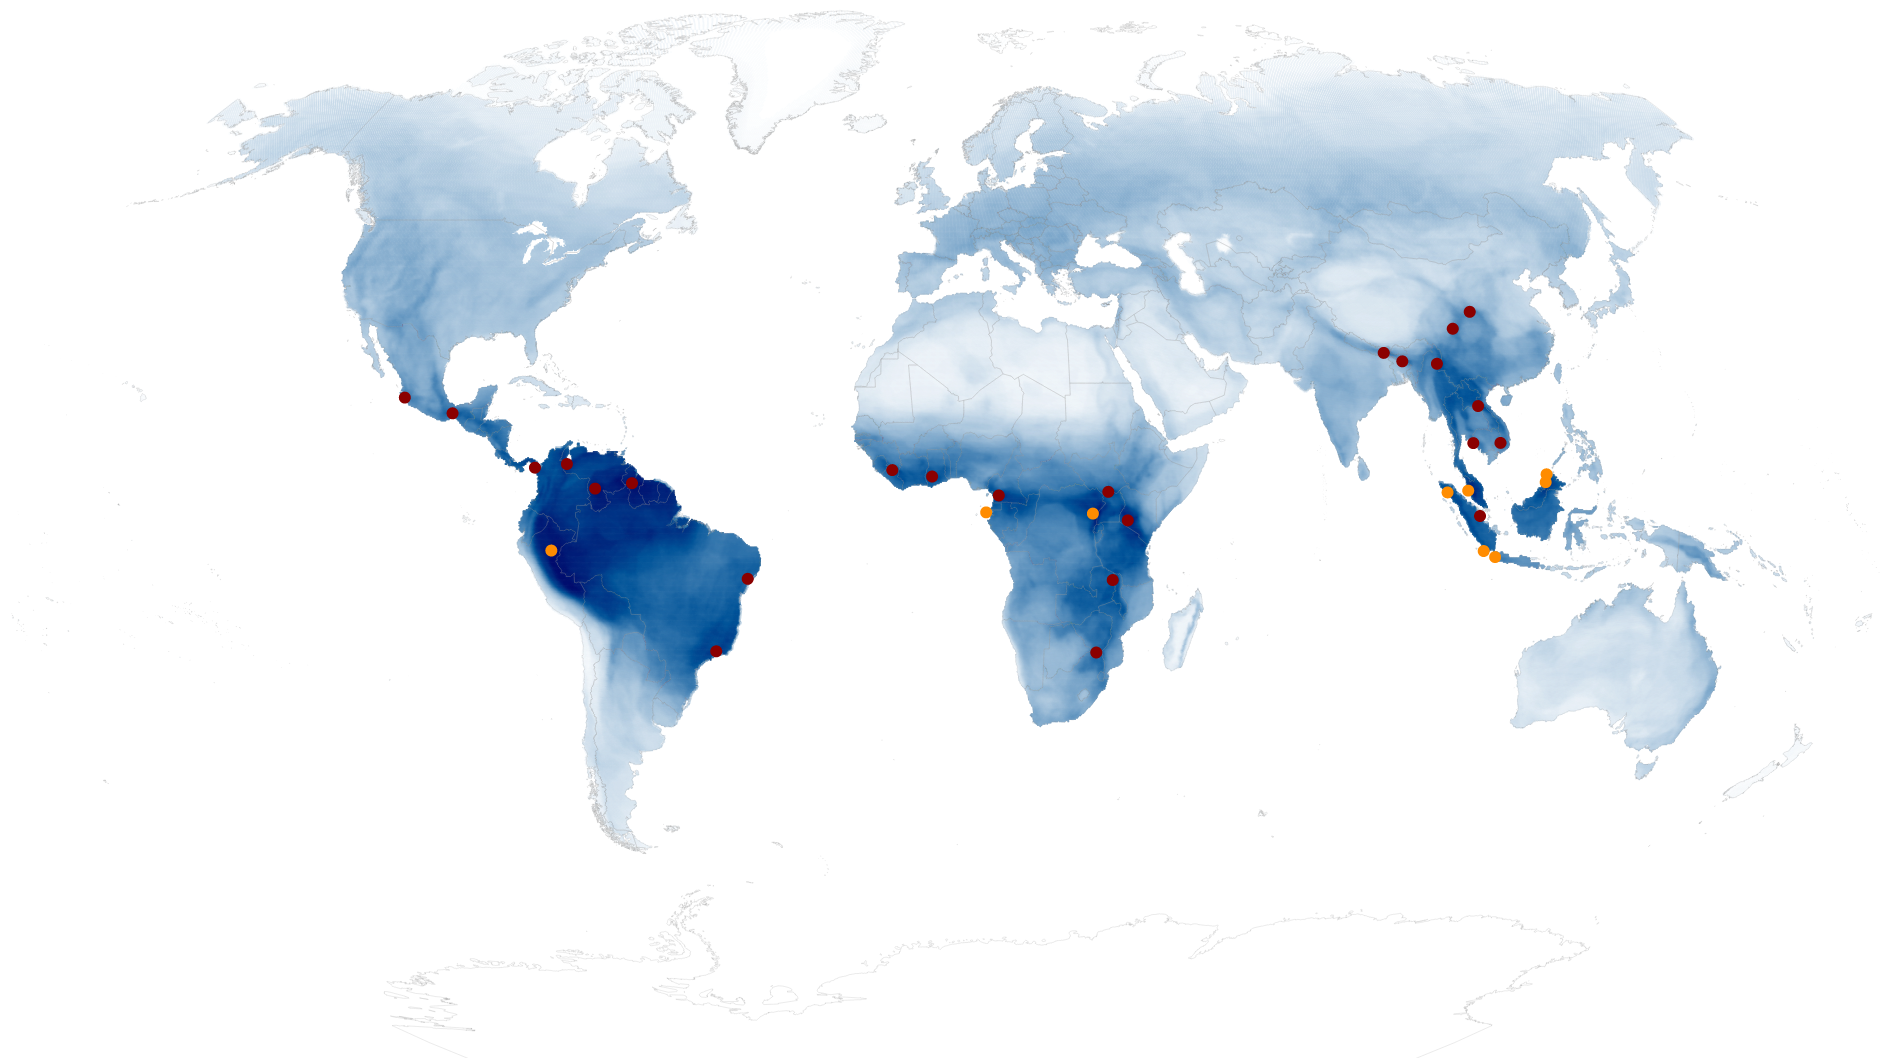
\includegraphics[width=17cm]{map.png}
			\caption{Heat map showing mammal density. Generated from depth of points on a grid overlaying the earth.}
		\end{figure}
		
		\begin{figure}[H]
			\centering
			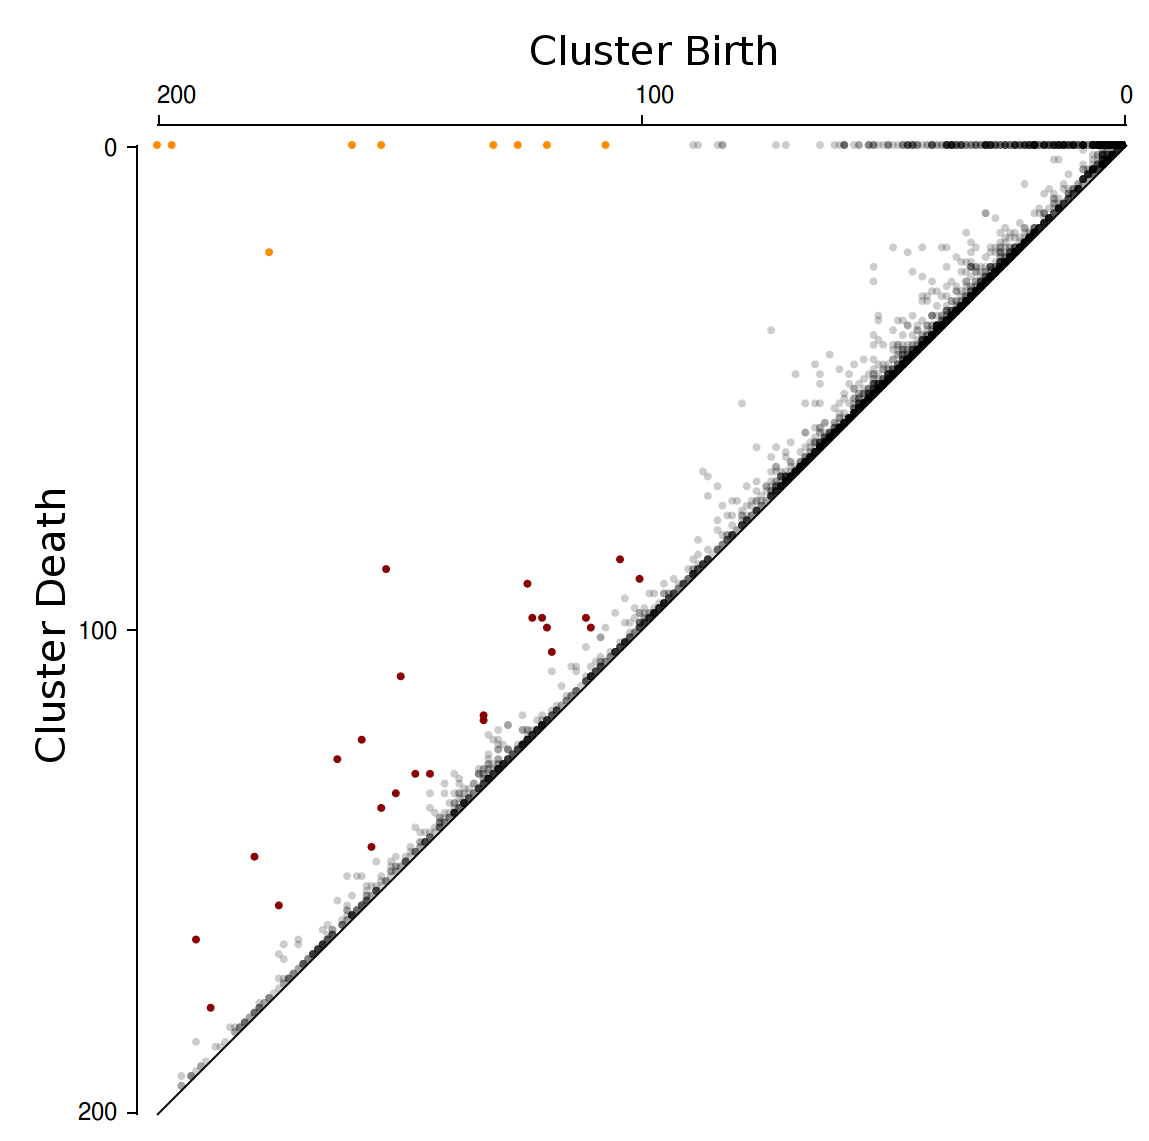
\includegraphics[width=8cm]{graph.png}
			\caption{Prominence diagram of mammal density. Orange points have both high density $>90$ and high prominence $>75$. Red points have high density $>90$ and prominence $<75$, but $>10$.}
		\end{figure}
		
	

		\pagebreak
	
	\section*{References}
		\beginrefs

			\bibentry{IUCN 17} International Union for the Conservation of Nature. (2017) \emph{Spatial Data Download}. Retrieved from http://www.iucnredlist.org/technical-documents/spatial-data/
			
			\bibentry{Jenkins 13} Jenkins, Clinton N. et al (2013). Global Patterns of Terrestrial Vertebrate Diversity and Conservation	\emph{PNAS}, vol. 110, no. 28. http://www.pnas.org/content/110/28/E2602.full

			\bibentry{Joshi 11} Joshi, D. (2011). Polygonal spatial clustering.  \emph{Computer Science and Engineering: Theses, Dissertations, and Student Research}, 16.
			
			\bibentry{Myers 00} Myers, Norman et al. (2000). Biodiversity Hotspots for Conservation Priorities	\emph{Nature}, vol. 403. http://www.nature.com/nature/journal/v403/n6772/full/403853a0.html
			
			\bibentry{Whuber 12} ``whuber'' from gis.stackexchange.com (2012). Answer to ``How Accurate is Approximating the Earth as a Sphere?''	\emph{stackexchange.com}, http://gis.stackexchange.com/a/25580. Accessed March, 2017. 


		\endrefs
	

		
		
	
	
\end{document}